\documentclass[12pt,a4paper]{article}

% ─── Packages ───────────────────────────────────────────────────
\usepackage[utf8]{inputenc}
\usepackage[T1]{fontenc}
\usepackage[margin=1in]{geometry}
\usepackage{amsmath,amssymb,amsthm,mathtools}
\usepackage{hyperref}
\usepackage{cleveref}
\usepackage{tikz-cd}
\usepackage{tikz}
\usetikzlibrary{positioning,arrows.meta,decorations.markings,calc,shapes,backgrounds,fit}
\usepackage{enumitem}
\usepackage{xcolor}
\usepackage{fancyhdr}
\usepackage{everypage}
\usepackage{abstract}
\usepackage{booktabs}
\usepackage{float}
\usepackage{setspace}
\usepackage{caption}
\usepackage{listings}

% ─── GrokRxiv DOI Sidebar ──────────────────────────────────────
\definecolor{grokgray}{RGB}{110,110,110}
\AddEverypageHook{%
  \ifnum\value{page}=1
    \begin{tikzpicture}[remember picture, overlay]
      \node[rotate=90, anchor=south, font=\Large\sffamily\bfseries\color{grokgray}, inner sep=0pt]
      at ([xshift=38pt, yshift=0.52\paperheight]current page.south west)
      {GrokRxiv:2026.03.dna-lang-typed-bio-programming\quad [\,bio.PL\,]\quad 31 Mar 2026};
    \end{tikzpicture}
  \fi
}

% ─── Theorem Environments ──────────────────────────────────────
\newtheorem{theorem}{Theorem}[section]
\newtheorem{lemma}[theorem]{Lemma}
\newtheorem{proposition}[theorem]{Proposition}
\newtheorem{corollary}[theorem]{Corollary}
\newtheorem{definition}[theorem]{Definition}
\newtheorem{example}[theorem]{Example}
\newtheorem{remark}[theorem]{Remark}
\newtheorem{axiom}[theorem]{Axiom}

% ─── Listings ──────────────────────────────────────────────────
\definecolor{codegreen}{RGB}{40,140,40}
\definecolor{codegray}{RGB}{100,100,100}
\definecolor{codepurple}{RGB}{120,50,160}
\definecolor{backcolour}{RGB}{248,248,248}
\definecolor{codeblue}{RGB}{30,80,180}

\lstdefinestyle{haskellstyle}{
    backgroundcolor=\color{backcolour},
    commentstyle=\color{codegreen}\itshape,
    keywordstyle=\color{codepurple}\bfseries,
    numberstyle=\tiny\color{codegray},
    stringstyle=\color{red!60!black},
    basicstyle=\ttfamily\small,
    breakatwhitespace=false,
    breaklines=true,
    captionpos=b,
    keepspaces=true,
    numbers=left,
    numbersep=5pt,
    showspaces=false,
    showstringspaces=false,
    showtabs=false,
    tabsize=2,
    language=Haskell,
    morekeywords={data,type,class,instance,where,deriving,newtype,module,import,qualified,as,do,let,in,case,of,if,then,else,forall}
}

\lstdefinestyle{dnalangstyle}{
    backgroundcolor=\color{backcolour},
    commentstyle=\color{codegreen}\itshape,
    keywordstyle=\color{codeblue}\bfseries,
    numberstyle=\tiny\color{codegray},
    stringstyle=\color{red!60!black},
    basicstyle=\ttfamily\small,
    breakatwhitespace=false,
    breaklines=true,
    captionpos=b,
    keepspaces=true,
    numbers=left,
    numbersep=5pt,
    showspaces=false,
    showstringspaces=false,
    showtabs=false,
    tabsize=2,
    morekeywords={program,target,sequence,guide,edit,vector,cell_line,assay,model_result,construct,candidate,require,run,collect,validate,log,return,let,DNA,RNA,Protein,Knockout,BaseEdit,PrimeEdit,Insertion,OffTarget,Toxicity,Immunogenicity,AND,OR,NOT}
}

\lstset{style=haskellstyle}

% ─── Custom Commands ───────────────────────────────────────────
\newcommand{\ie}{\textit{i.e.}}
\newcommand{\eg}{\textit{e.g.}}
\newcommand{\cf}{\textit{cf.}}
\newcommand{\DNALang}{\textsc{DNA-Lang}}
\newcommand{\ty}[1]{\texttt{#1}}
\newcommand{\kw}[1]{\textbf{\texttt{#1}}}

% ─── Page Style ────────────────────────────────────────────────
\pagestyle{fancy}
\fancyhf{}
\fancyhead[L]{\small\textit{DNA-Lang: A Typed Orchestration Language for Biological Programming}}
\fancyhead[R]{\small\thepage}
\renewcommand{\headrulewidth}{0.4pt}

% ═══════════════════════════════════════════════════════════════
% DOCUMENT
% ═══════════════════════════════════════════════════════════════

\begin{document}

\begin{center}
    {\LARGE\bfseries DNA-Lang: A Typed Orchestration Language\\[4pt] for Biological Programming}\\[18pt]
    {\large Matthew Long}\\[4pt]
    {\normalsize The YonedaAI Collaboration}\\
    {\normalsize Chicago, IL}\\[4pt]
    {\small\texttt{matt@yoneda.ai}}\\[18pt]
    {\normalsize Paper VIII in the series: \textit{DNA as a Programming Language}}\\[12pt]
    {\small March 31, 2026}
\end{center}

\begin{onecolabstract}
\noindent
We present \DNALang{}, a statically typed orchestration language that unifies seven biological data types---corresponding to the fundamental computational abstractions of the genome---with biotech workflow types for CRISPR editing, AI-driven protein engineering, experimental design, and regulatory compliance. The language provides a complete type system with refinement types for biological constraints, a four-layer compiler architecture producing design, AI, experiment, and compliance artifacts, and typed interfaces to AI models and CRISPR backends. We give the formal syntax, typing rules, and compilation semantics, prove type safety and compilation correctness, and provide a reference implementation in Haskell. The PCSK9 knockout therapy serves as a worked example demonstrating the full pipeline from program specification through type checking to artifact generation. \DNALang{} is the first programming language that treats the complete arc of biological intent---from target identification through experimental validation---as a single, type-checked program.
\end{onecolabstract}

\vspace{8pt}
\noindent\textbf{Keywords:} biological programming language, type system, CRISPR, gene editing, compiler, formal verification, biological computation, AI integration, provenance

\tableofcontents
\newpage

% ═══════════════════════════════════════════════════════════════
\section{Introduction}
\label{sec:intro}
% ═══════════════════════════════════════════════════════════════

Modern biotechnology operates with an abundance of powerful but disconnected tools. The Synthetic Biology Open Language (SBOL)~\cite{galdzicki2014sbol} provides a standard for biological design exchange. CRISPR-Cas systems~\cite{doudna2014crispr} enable precise genome editing. AI models such as AlphaFold~\cite{jumper2021alphafold} predict protein structures with near-experimental accuracy. Laboratory information management systems (LIMS) track experimental execution. Yet no unified, typed programming language spans the full arc from biological intent to experimental validation.

This gap has concrete consequences. A researcher designing a gene knockout must manually coordinate between sequence databases, guide RNA design tools, off-target prediction models, construct assembly protocols, cell line selection, assay design, and regulatory documentation. Each transition is untyped---a string passed from one tool to the next, with no compile-time guarantee that the output of one stage is a valid input to another.

In Papers I--VII of this series, we established that the genome itself is organized around seven distinct computational abstractions:

\begin{enumerate}[label=(\roman*)]
    \item \textbf{Coding sequences} as executable functions (Paper I): the central dogma as compilation from source (DNA) through intermediate representation (mRNA) to executable (protein).
    \item \textbf{Regulatory sequences} as control flow (Paper II): promoters, enhancers, silencers, and insulators implementing conditional execution, loops, and branching.
    \item \textbf{Non-coding RNA} as signals and middleware (Paper III): miRNA, siRNA, and lncRNA providing inter-process communication, message passing, and coordination.
    \item \textbf{Structural DNA} as memory layout (Paper IV): telomeres, centromeres, and topologically associating domains organizing the genome's address space.
    \item \textbf{Repetitive elements} as self-modifying code (Paper V): transposons, SINEs, and LINEs enabling runtime code rewriting and genomic plasticity.
    \item \textbf{Epigenetic marks} as runtime state (Paper VI): DNA methylation and histone modifications implementing mutable state that persists across cell divisions.
    \item \textbf{Developmental programs} as orchestration (Paper VII): Hox genes, morphogen gradients, and cell-fate networks composing the above into a coherent organism-level program.
\end{enumerate}

\DNALang{} synthesizes these seven biological types into a complete programming language, augmented with biotech workflow types that connect biological design to laboratory execution. The result is a language in which:

\begin{itemize}
    \item Every biological entity has a precise type.
    \item Every CRISPR editing operation is type-checked against its target.
    \item Every AI model invocation declares its input/output types, confidence bounds, and provenance.
    \item Every experimental step is traced from intent through execution to compliance documentation.
    \item The compiler produces not one artifact but four: a design artifact (SBOL-compatible sequences and constructs), an AI artifact (model predictions with uncertainty), an experiment artifact (assay plans with controls), and a compliance artifact (provenance and regulatory documentation).
\end{itemize}

The remainder of this paper is organized as follows. \Cref{sec:seven-types} summarizes the seven biological types. \Cref{sec:type-system} presents the unified type system. \Cref{sec:syntax} gives the complete syntax. \Cref{sec:type-checker} specifies the type checker. \Cref{sec:compiler} describes the four-layer compiler architecture. \Cref{sec:artifacts} details the four compiler artifacts. \Cref{sec:ai-service} formalizes AI as a typed service. \Cref{sec:crispr-backend} specifies the CRISPR backend. \Cref{sec:integration} describes integration points. \Cref{sec:example} presents the PCSK9 worked example. \Cref{sec:formal} states formal properties. \Cref{sec:implementation} describes the Haskell implementation. \Cref{sec:discussion} discusses implications and future work.


% ═══════════════════════════════════════════════════════════════
\section{The Seven Biological Types}
\label{sec:seven-types}
% ═══════════════════════════════════════════════════════════════

Each of the seven papers in this series identified a fundamental computational abstraction in the genome. \DNALang{} elevates each to a first-class type.

\subsection{ProteinCode\textlangle T\textrangle{} --- Executable Functions (Paper I)}

Coding sequences are the genome's functions. The central dogma---DNA $\to$ mRNA $\to$ protein---is a compilation pipeline: source code (the gene) is transcribed into an intermediate representation (mRNA), which is translated into an executable (the folded protein). The type \ty{ProteinCode\textlangle T\textrangle} parameterizes over the protein's functional class $T$ (enzyme, structural protein, transcription factor, etc.).

\begin{definition}[ProteinCode]
A value of type $\ty{ProteinCode}\langle T \rangle$ is a coding sequence that, when expressed, produces a protein of functional class $T$. The compilation pipeline is:
\[
\ty{ProteinCode}\langle T \rangle \xrightarrow{\text{transcription}} \ty{mRNA}\langle T \rangle \xrightarrow{\text{translation}} T
\]
\end{definition}

\subsection{Regulator\textlangle ExpressionLevel\textrangle{} --- Control Flow (Paper II)}

Regulatory sequences implement the genome's control flow. Promoters are function entry points. Enhancers are conditional jumps that activate expression when bound by specific transcription factors. Silencers are conditional blocks. Insulators are scope delimiters that prevent regulatory crosstalk.

\begin{definition}[Regulator]
A value of type $\ty{Regulator}\langle \text{ExpressionLevel} \rangle$ maps a set of transcription factor concentrations to an expression level:
\[
\ty{Regulator}\langle E \rangle : \text{TFContext} \to E
\]
where $E$ is a quantitative expression level in $[0, E_{\max}]$.
\end{definition}

\subsection{RNAControl\textlangle Process\textrangle{} --- Signals and Middleware (Paper III)}

Non-coding RNAs serve as the genome's signaling and middleware layer. MicroRNAs (miRNAs) act as message filters, silencing specific mRNAs post-transcriptionally. Small interfering RNAs (siRNAs) implement targeted message destruction. Long non-coding RNAs (lncRNAs) serve as scaffolds and coordinators, analogous to middleware buses.

\begin{definition}[RNAControl]
A value of type $\ty{RNAControl}\langle P \rangle$ modulates process $P$ through RNA-mediated regulation:
\[
\ty{RNAControl}\langle P \rangle : P \to P'
\]
where $P'$ is the post-regulation state of the process.
\end{definition}

\subsection{Structure\textlangle GenomeLayout\textrangle{} --- Memory Layout (Paper IV)}

Structural DNA elements organize the genome's three-dimensional architecture. Telomeres protect chromosome ends (buffer overflow guards). Centromeres enable chromosome segregation (memory allocation). Topologically associating domains (TADs) partition the genome into regulatory neighborhoods (memory segments).

\begin{definition}[Structure]
A value of type $\ty{Structure}\langle \text{GenomeLayout} \rangle$ defines a spatial organization of genomic regions:
\[
\ty{Structure}\langle G \rangle : \text{LinearGenome} \to \text{3DGenome}
\]
\end{definition}

\subsection{Repeat\textlangle SelfModifying\textrangle{} --- Self-Modifying Code (Paper V)}

Repetitive elements---transposons, SINEs, LINEs---are the genome's self-modifying code. Transposons copy or move themselves within the genome, rewriting the program at runtime. This enables genomic plasticity, immune system diversity (V(D)J recombination), and evolutionary innovation.

\begin{definition}[Repeat]
A value of type $\ty{Repeat}\langle \text{SelfModifying} \rangle$ is a genomic element capable of altering the genome:
\[
\ty{Repeat}\langle S \rangle : \text{Genome} \to \text{Genome}'
\]
where $\text{Genome}'$ differs from $\text{Genome}$ by the insertion, deletion, or rearrangement mediated by the element.
\end{definition}

\subsection{State\textlangle Accessibility\textrangle{} --- Runtime State (Paper VI)}

Epigenetic marks---DNA methylation, histone modifications---constitute the genome's mutable runtime state. Unlike the DNA sequence itself (the program text), epigenetic marks can be written and erased during execution (cell life). They determine which regions of the genome are accessible (open chromatin) or silenced (heterochromatin).

\begin{definition}[State]
A value of type $\ty{State}\langle \text{Accessibility} \rangle$ maps genomic loci to accessibility states:
\[
\ty{State}\langle A \rangle : \text{Locus} \to A
\]
where $A \in \{\text{Open}, \text{Poised}, \text{Repressed}, \text{Silent}\}$.
\end{definition}

\subsection{Program\textlangle OrganismDevelopment\textrangle{} --- Orchestration (Paper VII)}

Developmental programs---Hox gene cascades, morphogen gradients, cell-fate decision networks---orchestrate all previous types into a coherent organism-level computation. They are the genome's ``main function,'' composing functions, control flow, signals, memory layout, self-modification, and state into the emergent phenomenon of development.

\begin{definition}[Program]
A value of type $\ty{Program}\langle \text{OrganismDevelopment} \rangle$ is a composition of all six preceding types:
\[
\ty{Program}\langle O \rangle = (\ty{ProteinCode}, \ty{Regulator}, \ty{RNAControl}, \ty{Structure}, \ty{Repeat}, \ty{State}) \to O
\]
where $O$ is the developmental outcome (cell type, tissue, organ, organism).
\end{definition}

\begin{figure}[H]
\centering
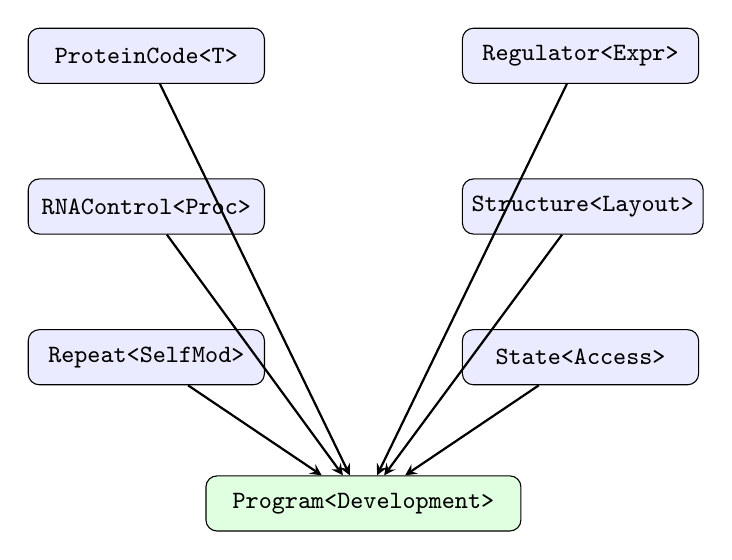
\begin{tikzpicture}[
    node distance=1.2cm and 2cm,
    typebox/.style={rectangle, draw, rounded corners, minimum width=3cm, minimum height=0.7cm, fill=blue!8, font=\small\ttfamily},
    arrow/.style={->, thick, >=stealth}
]
\node[typebox] (pc) {ProteinCode<T>};
\node[typebox, right=2.5cm of pc] (reg) {Regulator<Expr>};
\node[typebox, below=of pc] (rna) {RNAControl<Proc>};
\node[typebox, right=2.5cm of rna] (str) {Structure<Layout>};
\node[typebox, below=of rna] (rep) {Repeat<SelfMod>};
\node[typebox, right=2.5cm of rep] (sta) {State<Access>};
\node[typebox, below=1.5cm of $(rep)!0.5!(sta)$, fill=green!12, minimum width=4cm] (prog) {Program<Development>};

\draw[arrow] (pc) -- (prog);
\draw[arrow] (reg) -- (prog);
\draw[arrow] (rna) -- (prog);
\draw[arrow] (str) -- (prog);
\draw[arrow] (rep) -- (prog);
\draw[arrow] (sta) -- (prog);
\end{tikzpicture}
\caption{The seven biological types. \ty{Program} composes all six preceding types into organism-level orchestration.}
\label{fig:seven-types}
\end{figure}


% ═══════════════════════════════════════════════════════════════
\section{The Unified Type System}
\label{sec:type-system}
% ═══════════════════════════════════════════════════════════════

The \DNALang{} type system extends the seven biological types with biotech workflow types, refinement types, and a composite genome type.

\subsection{Core Types}

\begin{definition}[Core Type Universe]
The set of \DNALang{} types $\mathcal{T}$ is defined by the grammar:
\begin{align*}
\tau ::=\; & \ty{ProteinCode} \mid \ty{Regulator} \mid \ty{RNAControl} \mid \ty{Structure} \mid \ty{Repeat} \mid \ty{State} \mid \ty{Program} \\
\mid\; & \ty{Target} \mid \ty{Sequence}\langle \kappa \rangle \mid \ty{GuideRNA} \mid \ty{Edit}\langle \epsilon \rangle \mid \ty{Vector} \mid \ty{CellLine} \\
\mid\; & \ty{Assay} \mid \ty{Phenotype} \mid \ty{Candidate} \mid \ty{Risk}\langle \rho \rangle \mid \ty{Evidence} \mid \ty{Workflow} \\
\mid\; & \{\tau \mid \phi\} \mid \ty{Genome} \mid [\tau] \mid (\tau_1, \ldots, \tau_n) \to \tau \\[4pt]
\kappa ::=\; & \ty{DNA} \mid \ty{RNA} \mid \ty{Protein} \\
\epsilon ::=\; & \ty{Knockout} \mid \ty{BaseEdit} \mid \ty{PrimeEdit} \mid \ty{Insertion} \\
\rho ::=\; & \ty{OffTarget} \mid \ty{Toxicity} \mid \ty{Immunogenicity}
\end{align*}
\end{definition}

\subsection{Biotech Workflow Types}

The workflow types model the stages of a biotech pipeline:

\begin{table}[H]
\centering
\caption{Biotech workflow types and their biological interpretation.}
\label{tab:workflow-types}
\begin{tabular}{lll}
\toprule
\textbf{Type} & \textbf{Description} & \textbf{Analogy} \\
\midrule
\ty{Target}              & Gene or locus to modify     & Function pointer \\
\ty{Sequence$\langle\kappa\rangle$} & DNA, RNA, or protein sequence & Data buffer \\
\ty{GuideRNA}            & CRISPR guide RNA            & Instruction operand \\
\ty{Edit$\langle\epsilon\rangle$}   & Editing operation           & Write instruction \\
\ty{Vector}              & Delivery vehicle            & Network packet \\
\ty{CellLine}            & Experimental cell system    & Execution environment \\
\ty{Assay}               & Experimental measurement    & Test harness \\
\ty{Phenotype}           & Observed outcome            & Program output \\
\ty{Candidate}           & Therapeutic candidate       & Release artifact \\
\ty{Risk$\langle\rho\rangle$}      & Safety assessment           & Error report \\
\ty{Evidence}            & Supporting data             & Log entry \\
\ty{Workflow}            & Pipeline composition        & Build script \\
\bottomrule
\end{tabular}
\end{table}

\subsection{Refinement Types}

Refinement types attach biological constraints to base types. A refinement type $\{\tau \mid \phi\}$ denotes values of type $\tau$ satisfying predicate $\phi$.

\begin{definition}[Biological Constraints]
The constraint language $\phi$ is:
\begin{align*}
\phi ::=\; & \texttt{length} \geq n \mid \texttt{length} \leq n \\
\mid\; & l \leq \texttt{GC} \leq h \mid \texttt{off\_targets} = 0 \\
\mid\; & \texttt{specificity} \geq s \mid \texttt{efficiency} \geq e \\
\mid\; & \texttt{risk}(\rho) \leq v \mid \texttt{PAM} = p \\
\mid\; & l \leq \texttt{expression} \leq h \\
\mid\; & \phi_1 \wedge \phi_2 \mid \phi_1 \vee \phi_2 \mid \neg \phi \mid \top
\end{align*}
\end{definition}

\begin{example}[Refined GuideRNA]
A guide RNA with specificity at least 0.9 and no off-targets:
\[
\ty{SafeGuide} = \{\ty{GuideRNA} \mid \texttt{specificity} \geq 0.9 \wedge \texttt{off\_targets} = 0\}
\]
\end{example}

\subsection{The Genome Composite Type}

The \ty{Genome} type is the composite of all seven biological types:

\begin{definition}[Genome]
\[
\ty{Genome} = \ty{ProteinCode} \times \ty{Regulator} \times \ty{RNAControl} \times \ty{Structure} \times \ty{Repeat} \times \ty{State} \times \ty{Program}
\]
Every biological type is a subtype of \ty{Genome}: for each $\tau \in \{\ty{ProteinCode}, \ldots, \ty{Program}\}$, we have $\tau <: \ty{Genome}$.
\end{definition}

\subsection{Subtyping}

\begin{definition}[Subtyping Rules]
The subtyping relation $<:$ is the smallest reflexive and transitive relation satisfying:
\begin{enumerate}[label=(\alph*)]
    \item $\tau <: \tau$ (reflexivity)
    \item $\{\tau \mid \phi\} <: \tau$ (refinement subsumption)
    \item $\tau_{\text{bio}} <: \ty{Genome}$ for each biological type $\tau_{\text{bio}}$
    \item $\ty{GuideRNA} <: \ty{Sequence}\langle\ty{DNA}\rangle$ (a guide is a DNA sequence)
    \item $\ty{Candidate} <: \ty{Evidence}$ (a candidate is evidence)
    \item $[\tau_1] <: [\tau_2]$ if $\tau_1 <: \tau_2$ (list covariance)
\end{enumerate}
\end{definition}


% ═══════════════════════════════════════════════════════════════
\section{DNA-Lang Syntax}
\label{sec:syntax}
% ═══════════════════════════════════════════════════════════════

\subsection{Program Structure}

A \DNALang{} program consists of a named program block containing declarations and actions:

\begin{lstlisting}[style=dnalangstyle,caption={General program structure.},label={lst:structure}]
program <Name> {
    <declarations>
    <actions>
}
\end{lstlisting}

Declarations introduce typed bindings. Actions perform side-effecting operations (running assays, collecting results, validating constraints).

\subsection{Declarations}

\begin{definition}[Declaration Forms]
\DNALang{} supports the following declaration forms:
\begin{align*}
d ::=\; & \kw{target}\; x = e \\
\mid\; & \kw{sequence}\; x : \kappa = e \\
\mid\; & \kw{guide}\; x = e \\
\mid\; & \kw{edit}\; x : \epsilon = e \\
\mid\; & \kw{vector}\; x = e \\
\mid\; & \kw{cell\_line}\; x = e \\
\mid\; & \kw{assay}\; x = e \\
\mid\; & \kw{model\_result}\; x = e \\
\mid\; & \kw{construct}\; x = e \\
\mid\; & \kw{candidate}\; x = e \\
\mid\; & \kw{let}\; x : \tau = e \\
\mid\; & \kw{require}\; \phi
\end{align*}
\end{definition}

Each declaration introduces a binding $x$ of the appropriate type into the type environment, with the exception of \kw{require}, which asserts a constraint $\phi$ that must hold at compile time.

\subsection{Expressions}

\begin{definition}[Expression Forms]
\begin{align*}
e ::=\; & x \mid \text{``}s\text{''} \mid n \mid f \mid \texttt{true} \mid \texttt{false} \\
\mid\; & [e_1, \ldots, e_n] \mid \{k_1 = e_1, \ldots, k_n = e_n\} \\
\mid\; & g(e_1, \ldots, e_n) \mid e.k \mid e_1 \oplus e_2 \mid e : \tau
\end{align*}
where $x$ is a variable, $s$ a string, $n$ an integer, $f$ a float, $g$ a function name, $k$ a field name, $\oplus$ a binary operator, and $\tau$ a type annotation.
\end{definition}

\subsection{Actions}

\begin{definition}[Action Forms]
\begin{align*}
a ::=\; & \kw{run}\; g(e_1, \ldots, e_n) \\
\mid\; & \kw{collect}\; x = e \\
\mid\; & \kw{validate}\; e \\
\mid\; & \kw{log}\; e \\
\mid\; & \kw{return}\; e
\end{align*}
\end{definition}

\subsection{Full Grammar}

\begin{figure}[H]
\centering
\begin{minipage}{0.95\textwidth}
\begin{align*}
\textit{program} &::= \kw{program}\; \textit{name}\; \texttt{\{}\; \textit{item}^*\; \texttt{\}} \\
\textit{item} &::= \textit{decl} \mid \textit{action} \\
\textit{decl} &::= \kw{target}\; \textit{name}\; \texttt{=}\; \textit{expr} \\
    &\mid\; \kw{sequence}\; \textit{name}\; \texttt{:}\; \textit{seqkind}\; \texttt{=}\; \textit{expr} \\
    &\mid\; \kw{guide}\; \textit{name}\; \texttt{=}\; \textit{expr} \\
    &\mid\; \kw{edit}\; \textit{name}\; \texttt{:}\; \textit{editkind}\; \texttt{=}\; \textit{expr} \\
    &\mid\; \kw{require}\; \textit{constraint} \\
    &\mid\; \ldots \\
\textit{expr} &::= \textit{name} \mid \textit{literal} \mid \textit{name}\texttt{(}\textit{expr}^{*}\texttt{)} \mid \textit{expr}\texttt{.}\textit{name} \mid \texttt{[}\textit{expr}^{*}\texttt{]} \mid \texttt{\{}\textit{fields}\texttt{\}} \\
\textit{action} &::= \kw{run}\; \textit{name}\texttt{(}\textit{expr}^{*}\texttt{)} \mid \kw{collect}\; \textit{name}\; \texttt{=}\; \textit{expr} \mid \ldots \\
\textit{seqkind} &::= \ty{DNA} \mid \ty{RNA} \mid \ty{Protein} \\
\textit{editkind} &::= \ty{Knockout} \mid \ty{BaseEdit} \mid \ty{PrimeEdit} \mid \ty{Insertion} \\
\textit{constraint} &::= \texttt{no\_off\_targets} \mid \texttt{specificity} \geq f \mid \texttt{efficiency} \geq f \mid \ldots
\end{align*}
\end{minipage}
\caption{Abbreviated grammar for \DNALang{}.}
\label{fig:grammar}
\end{figure}


% ═══════════════════════════════════════════════════════════════
\section{The Type Checker}
\label{sec:type-checker}
% ═══════════════════════════════════════════════════════════════

\subsection{Typing Judgments}

The type checker maintains a type environment $\Gamma : \text{Name} \to \mathcal{T}$ and checks each declaration and action in sequence.

\begin{definition}[Typing Judgment]
The judgment $\Gamma \vdash e : \tau$ means ``in environment $\Gamma$, expression $e$ has type $\tau$.''
\end{definition}

\subsection{Typing Rules for Expressions}

\begin{gather}
\frac{x : \tau \in \Gamma}{\Gamma \vdash x : \tau} \quad \textsc{(Var)}
\qquad
\frac{}{\Gamma \vdash \text{``}s\text{''} : \ty{String}} \quad \textsc{(Str)}
\qquad
\frac{}{\Gamma \vdash n : \ty{Int}} \quad \textsc{(Int)}
\\[8pt]
\frac{g : (\tau_1, \ldots, \tau_n) \to \tau_r \quad \Gamma \vdash e_i : \tau_i' \quad \tau_i' <: \tau_i \;\forall i}{\Gamma \vdash g(e_1, \ldots, e_n) : \tau_r} \quad \textsc{(App)}
\\[8pt]
\frac{\Gamma \vdash e_1 : \tau \quad \ldots \quad \Gamma \vdash e_n : \tau}{\Gamma \vdash [e_1, \ldots, e_n] : [\tau]} \quad \textsc{(List)}
\qquad
\frac{\Gamma \vdash e : \tau \quad \tau <: \tau'}{\Gamma \vdash e : \tau'} \quad \textsc{(Sub)}
\end{gather}

\subsection{Typing Rules for Declarations}

\begin{gather}
\frac{\Gamma \vdash e : \tau}{\Gamma \vdash (\kw{target}\; x = e) \Rightarrow \Gamma[x \mapsto \ty{Target}]} \quad \textsc{(Target)}
\\[8pt]
\frac{\Gamma \vdash e : \tau \quad \tau <: \ty{Sequence}\langle\kappa\rangle}{\Gamma \vdash (\kw{sequence}\; x : \kappa = e) \Rightarrow \Gamma[x \mapsto \ty{Sequence}\langle\kappa\rangle]} \quad \textsc{(Seq)}
\\[8pt]
\frac{\Gamma \vdash e : \tau \quad \tau <: \ty{GuideRNA}}{\Gamma \vdash (\kw{guide}\; x = e) \Rightarrow \Gamma[x \mapsto \ty{GuideRNA}]} \quad \textsc{(Guide)}
\\[8pt]
\frac{\Gamma \vdash e : \ty{Edit}\langle\epsilon'\rangle \quad \epsilon' <: \epsilon}{\Gamma \vdash (\kw{edit}\; x : \epsilon = e) \Rightarrow \Gamma[x \mapsto \ty{Edit}\langle\epsilon\rangle]} \quad \textsc{(Edit)}
\\[8pt]
\frac{\Gamma \vdash \phi \;\text{valid}}{\Gamma \vdash (\kw{require}\; \phi) \Rightarrow \Gamma} \quad \textsc{(Require)}
\end{gather}

\subsection{Refinement Type Checking}

When a \kw{require} constraint is encountered, the type checker validates it against the constraint language. At compile time, this performs structural validation (non-negative lengths, valid GC ranges, etc.). At link time---when concrete sequences are available---refinement predicates are evaluated against the actual data.

\begin{definition}[Constraint Validity]
A constraint $\phi$ is \emph{structurally valid} if:
\begin{itemize}
    \item $\texttt{length} \geq n$ with $n \geq 0$
    \item $l \leq \texttt{GC} \leq h$ with $0 \leq l \leq h \leq 1$
    \item $\texttt{specificity} \geq s$ with $0 \leq s \leq 1$
    \item $\texttt{risk}(\rho) \leq v$ with $v \geq 0$
    \item $\phi_1 \wedge \phi_2$ with both $\phi_1$ and $\phi_2$ valid
    \item $\top$ is always valid
\end{itemize}
\end{definition}

\subsection{Type Inference}

\DNALang{} uses bidirectional type checking. Declarations provide type annotations (the sequence kind $\kappa$, the edit kind $\epsilon$), and expressions are checked against these annotations. Function applications infer return types from the built-in function signature table.


% ═══════════════════════════════════════════════════════════════
\section{The Compiler Architecture --- Four Layers}
\label{sec:compiler}
% ═══════════════════════════════════════════════════════════════

The \DNALang{} compiler is organized into four layers, each transforming the program closer to executable artifacts.

\begin{figure}[H]
\centering
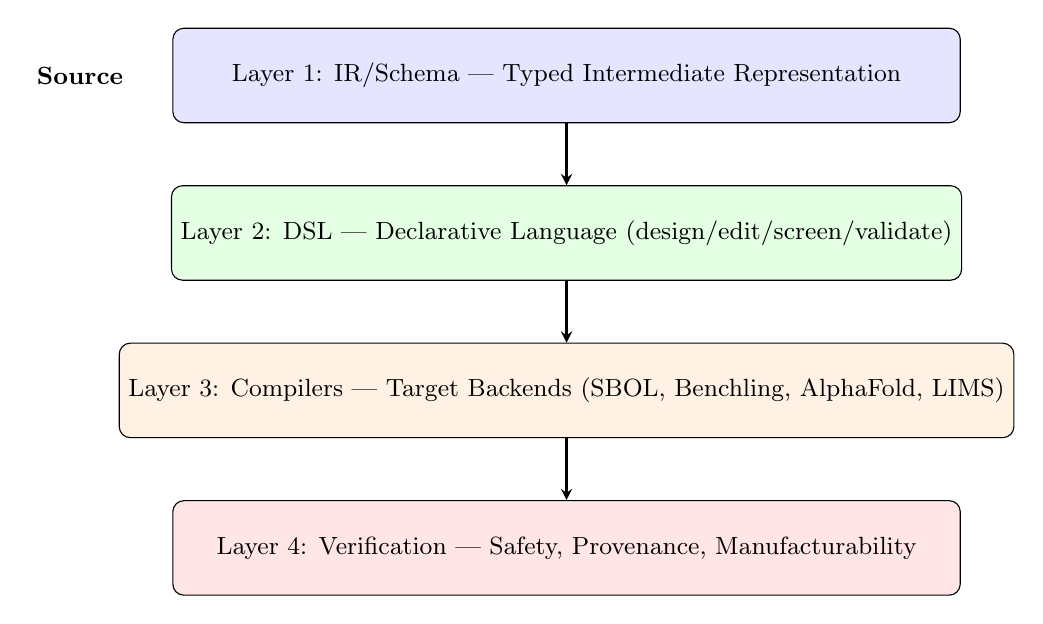
\begin{tikzpicture}[
    layer/.style={rectangle, draw, rounded corners, minimum width=10cm, minimum height=1.2cm, fill=#1, font=\small},
    arrow/.style={->, thick, >=stealth}
]
\node[layer=blue!10]   (l1) at (0,0)    {Layer 1: IR/Schema --- Typed Intermediate Representation};
\node[layer=green!10]  (l2) at (0,-2)   {Layer 2: DSL --- Declarative Language (design/edit/screen/validate)};
\node[layer=orange!10] (l3) at (0,-4)   {Layer 3: Compilers --- Target Backends (SBOL, Benchling, AlphaFold, LIMS)};
\node[layer=red!10]    (l4) at (0,-6)   {Layer 4: Verification --- Safety, Provenance, Manufacturability};

\node[left=0.5cm of l1, font=\small\bfseries] {Source};

\draw[arrow] (l1) -- (l2);
\draw[arrow] (l2) -- (l3);
\draw[arrow] (l3) -- (l4);
\end{tikzpicture}
\caption{The four-layer compiler architecture.}
\label{fig:compiler-layers}
\end{figure}

\subsection{Layer 1: IR/Schema}

The first layer lowers the parsed \DNALang{} AST into a typed intermediate representation (IR). Every node in the IR carries its type annotation, enabling downstream passes to perform type-directed transformations without re-running the type checker.

The IR preserves the program's declaration order, which matters because biological workflows are inherently sequential: a guide cannot be designed before its target is specified.

\subsection{Layer 2: DSL}

The second layer interprets the IR as a declarative specification in four domains:
\begin{enumerate}
    \item \textbf{Design}: target identification, sequence retrieval, guide design, construct assembly.
    \item \textbf{Edit}: CRISPR operation specification (knockout, base edit, prime edit, insertion).
    \item \textbf{Screen}: assay design, cell line selection, phenotype measurement.
    \item \textbf{Validate}: safety checks, off-target analysis, risk assessment.
\end{enumerate}

\subsection{Layer 3: Compilers}

The third layer compiles the domain-specific representations to concrete external formats:
\begin{itemize}
    \item \textbf{SBOL 3.0}: biological design components, interactions, and modules.
    \item \textbf{Benchling API}: sequence entries, annotations, and assembly protocols.
    \item \textbf{AlphaFold 3}: structure prediction requests with input sequences and parameters.
    \item \textbf{LIMS/ELN}: experimental protocols, sample tracking, and instrument configurations.
\end{itemize}

\subsection{Layer 4: Verification}

The fourth layer performs cross-cutting verification:
\begin{itemize}
    \item \textbf{Off-target analysis}: genome-wide search for guide RNA binding sites.
    \item \textbf{Payload verification}: construct size, expression cassette integrity, codon optimization.
    \item \textbf{Manufacturability}: synthesis constraints, restriction site avoidance, GC content bounds.
    \item \textbf{Provenance}: complete trace from every output artifact back to its source declaration, through every model invocation and compilation step.
\end{itemize}


% ═══════════════════════════════════════════════════════════════
\section{Four Compiler Artifacts}
\label{sec:artifacts}
% ═══════════════════════════════════════════════════════════════

Compilation of a \DNALang{} program produces not one but four artifacts, each serving a distinct stakeholder.

\subsection{Design Artifact}

The design artifact contains everything needed to physically realize the intended biological modification:

\begin{itemize}
    \item Target gene annotation and genomic coordinates
    \item Reference and modified sequences in GenBank and SBOL XML formats
    \item Guide RNA sequences with PAM sites and scoring metrics
    \item Construct maps with assembly instructions (Gibson, Golden Gate, etc.)
    \item Edit plans specifying the mechanism (NHEJ, HDR, base editing, prime editing)
\end{itemize}

\subsection{AI Artifact}

The AI artifact documents every AI model invocation and its outputs:

\begin{itemize}
    \item Model identity and version (AlphaFold 3 release 2025-12, ESM-2 650M, etc.)
    \item Input hashes for reproducibility
    \item Predictions with calibrated confidence scores
    \item Uncertainty estimates (MC Dropout, Deep Ensemble)
    \item Ranking criteria and composite scores for guide selection
\end{itemize}

\subsection{Experiment Artifact}

The experiment artifact is a complete, executable experimental plan:

\begin{itemize}
    \item Assay protocols with step-by-step instructions
    \item Cell line specifications with authentication and passage requirements
    \item Controls: positive (known-functional guide), negative (scrambled guide), untransfected
    \item Statistical plan: sample size, replicates, tests, significance thresholds
    \item Acceptance criteria: minimum editing efficiency, maximum off-target rate
    \item Timeline with milestones (transfection, harvest, analysis, reporting)
\end{itemize}

\subsection{Compliance Artifact}

The compliance artifact provides regulatory and audit documentation:

\begin{itemize}
    \item Complete provenance chain from source code to every output
    \item Type environment snapshot at compilation
    \item All constraint verifications with pass/fail status
    \item Model version registry with checksums
    \item Decision log recording every automated choice with rationale
    \item Regulatory classification and biosafety level
    \item Audit trail with timestamps and compiler version
\end{itemize}


% ═══════════════════════════════════════════════════════════════
\section{AI as Typed Service}
\label{sec:ai-service}
% ═══════════════════════════════════════════════════════════════

In \DNALang{}, AI models are not opaque black boxes but typed services with declared interfaces. Each AI function has:

\begin{enumerate}
    \item A \textbf{type signature}: input and output types.
    \item A \textbf{confidence bound}: calibrated probability that the prediction is correct within a specified tolerance.
    \item A \textbf{provenance record}: model identity, version, checkpoint hash, and input hash.
    \item A \textbf{validation protocol}: how to experimentally verify the prediction.
\end{enumerate}

\begin{definition}[AI Service Signatures]
The built-in AI services are:
\begin{align*}
\texttt{predict\_structure} &: \ty{Sequence}\langle\ty{Protein}\rangle \to \ty{Structure} \\
\texttt{rank\_guides} &: \ty{Target} \to [\ty{GuideRNA}] \\
\texttt{predict\_off\_target} &: \ty{GuideRNA} \to \ty{Risk}\langle\ty{OffTarget}\rangle \\
\texttt{propose\_variants} &: \ty{Sequence}\langle\ty{Protein}\rangle \to [\ty{Sequence}\langle\ty{Protein}\rangle]
\end{align*}
\end{definition}

\begin{example}[Typed AI Invocation]
When the program calls \texttt{predict\_structure(seq)}, the type checker verifies that \texttt{seq} has type $\ty{Sequence}\langle\ty{Protein}\rangle$. The return type $\ty{Structure}$ is guaranteed. The AI artifact records the model version, input hash, pLDDT scores, and PAE matrix.
\end{example}

The key principle is that \emph{AI uncertainty is a first-class citizen of the type system}. A structure prediction does not simply return a PDB file; it returns a $\ty{Structure}$ value annotated with confidence metrics that downstream consumers can inspect and branch on.

\begin{remark}
The typed AI service approach addresses a critical gap in current biotech workflows: the tendency to treat AI predictions as ground truth. By requiring explicit confidence bounds and validation protocols, \DNALang{} forces researchers to acknowledge and plan for prediction uncertainty.
\end{remark}


% ═══════════════════════════════════════════════════════════════
\section{CRISPR as Backend}
\label{sec:crispr-backend}
% ═══════════════════════════════════════════════════════════════

CRISPR-Cas systems serve as the primary execution backend for \DNALang{} programs. Each editing modality is a typed operation that compiles to concrete molecular components.

\subsection{Editing Operations}

\begin{definition}[CRISPR Operations]
\begin{align*}
\texttt{knockout} &: (\ty{Target}, \ty{GuideRNA}) \to \ty{Edit}\langle\ty{Knockout}\rangle \\
\texttt{base\_edit} &: (\ty{Target}, \ty{GuideRNA}, \ty{Sequence}\langle\ty{DNA}\rangle) \to \ty{Edit}\langle\ty{BaseEdit}\rangle \\
\texttt{prime\_edit} &: (\ty{Target}, \ty{GuideRNA}, \ty{Sequence}\langle\ty{DNA}\rangle) \to \ty{Edit}\langle\ty{PrimeEdit}\rangle \\
\texttt{insert\_payload} &: (\ty{Target}, \ty{GuideRNA}, \ty{Sequence}\langle\ty{DNA}\rangle) \to \ty{Edit}\langle\ty{Insertion}\rangle
\end{align*}
\end{definition}

\subsection{Compilation to Molecular Components}

Each CRISPR operation compiles to a set of molecular components:

\begin{table}[H]
\centering
\caption{CRISPR operations and their compiled molecular components.}
\label{tab:crispr-compilation}
\begin{tabular}{lp{9cm}}
\toprule
\textbf{Operation} & \textbf{Compiled Components} \\
\midrule
\texttt{knockout} & SpCas9 protein or mRNA, guide RNA with scaffold, delivery vehicle (RNP, LNP, or AAV) \\
\texttt{base\_edit} & ABE8e or CBE4 fusion protein, guide RNA, no donor template required \\
\texttt{prime\_edit} & PE2 or PE3 nickase fusion, pegRNA with primer binding site and RT template, nicking guide \\
\texttt{insert\_payload} & SpCas9, guide RNA, HDR donor template with homology arms (typically 500--1000bp each), delivery vehicle \\
\bottomrule
\end{tabular}
\end{table}

\subsection{Additional CRISPR Modalities}

Beyond the four core editing operations, \DNALang{} supports CRISPRa (activation) and CRISPRi (repression) as typed operations:

\begin{align*}
\texttt{activate} &: (\ty{Target}, \ty{GuideRNA}) \to \ty{Edit}\langle\ty{Insertion}\rangle \\
\texttt{repress} &: (\ty{Target}, \ty{GuideRNA}) \to \ty{Edit}\langle\ty{Knockout}\rangle
\end{align*}

These compile to dCas9 fusion proteins (VP64, p65, Rta for activation; KRAB for repression) with the specified guide RNA.


% ═══════════════════════════════════════════════════════════════
\section{Integration Points}
\label{sec:integration}
% ═══════════════════════════════════════════════════════════════

\DNALang{} is designed to integrate with existing biotech infrastructure rather than replace it.

\subsection{SBOL (Synthetic Biology Open Language)}

The design artifact exports biological components, interactions, and modules in SBOL 3.0 format. Each \ty{Sequence} declaration maps to an SBOL \texttt{Component}. Each \ty{Edit} maps to an SBOL \texttt{Interaction}. The program's declaration structure maps to an SBOL \texttt{Module} hierarchy.

\subsection{Benchling}

Benchling integration provides sequence management, annotation, and collaboration. The \DNALang{} compiler generates Benchling API calls to:
\begin{itemize}
    \item Create and annotate sequences
    \item Register constructs with assembly protocols
    \item Track guide RNA designs with scoring metrics
    \item Link experimental results to design specifications
\end{itemize}

\subsection{AlphaFold 3}

Structure prediction requests are compiled into AlphaFold 3 API calls with:
\begin{itemize}
    \item Input sequences in the required format
    \item Multimer specifications for protein complexes
    \item Post-processing to extract pLDDT, PAE, and contact maps
    \item Caching of results keyed by input sequence hash
\end{itemize}

\subsection{LIMS/ELN}

Laboratory execution is managed through LIMS integration:
\begin{itemize}
    \item Experimental protocols generated from assay declarations
    \item Sample registration and tracking
    \item Instrument configuration and scheduling
    \item Result capture and automated quality control
    \item Notebook entries linked to program source and compilation artifacts
\end{itemize}


% ═══════════════════════════════════════════════════════════════
\section{Worked Example: PCSK9 Knockout Therapy}
\label{sec:example}
% ═══════════════════════════════════════════════════════════════

We now trace the complete \DNALang{} pipeline for a PCSK9 knockout therapy program. PCSK9 (Proprotein Convertase Subtilisin/Kexin Type 9) is a validated target for lowering LDL cholesterol; Verve Therapeutics' VERVE-101 demonstrated clinical proof-of-concept for in vivo base editing of PCSK9 in humans~\cite{verve2023}.

\subsection{The Program}

\begin{lstlisting}[style=dnalangstyle,caption={PCSK9 knockout therapy program in \DNALang{}.},label={lst:pcsk9}]
program PCSK9_KO {
    -- Target identification
    target pcsk9 = "PCSK9"
    sequence ref_seq : DNA = lookup_sequence(pcsk9)

    -- Guide RNA design
    guide top_guide = design_guide(pcsk9, ref_seq)

    -- Biological constraints
    require no_off_targets
    require specificity >= 0.90
    require efficiency >= 0.70

    -- CRISPR editing
    edit ko_edit : Knockout = knockout(pcsk9, top_guide)

    -- Experimental setup
    cell_line hepg2 = select_cell_line("HepG2")
    assay ngs_assay = design_assay(ko_edit, hepg2)

    -- Execution
    run validate_safety(ko_edit)
    run run_assay(ngs_assay, hepg2)
    collect results = generate_report(ngs_assay, ko_edit)
}
\end{lstlisting}

\subsection{Type Checking Trace}

The type checker processes each declaration in order, building the type environment:

\begin{enumerate}
    \item $\Gamma_0 = \emptyset$
    \item \kw{target} \texttt{pcsk9 = "PCSK9"}: The string literal has type \ty{String}. The \textsc{Target} rule extends: $\Gamma_1 = \Gamma_0[\texttt{pcsk9} \mapsto \ty{Target}]$.
    \item \kw{sequence} \texttt{ref\_seq : DNA = lookup\_sequence(pcsk9)}: The function \texttt{lookup\_sequence} has signature $\ty{Target} \to \ty{Sequence}\langle\ty{DNA}\rangle$. Since $\texttt{pcsk9} : \ty{Target} \in \Gamma_1$, the application type-checks. $\Gamma_2 = \Gamma_1[\texttt{ref\_seq} \mapsto \ty{Sequence}\langle\ty{DNA}\rangle]$.
    \item \kw{guide} \texttt{top\_guide = design\_guide(pcsk9, ref\_seq)}: The function \texttt{design\_guide} has signature $(\ty{Target}, \ty{Sequence}\langle\ty{DNA}\rangle) \to \ty{GuideRNA}$. Both arguments match. $\Gamma_3 = \Gamma_2[\texttt{top\_guide} \mapsto \ty{GuideRNA}]$.
    \item \kw{require} \texttt{no\_off\_targets}: Structurally valid. $\Gamma_4 = \Gamma_3$.
    \item \kw{require} \texttt{specificity >= 0.90}: $0 \leq 0.90 \leq 1$. Valid. $\Gamma_5 = \Gamma_4$.
    \item \kw{require} \texttt{efficiency >= 0.70}: $0 \leq 0.70 \leq 1$. Valid. $\Gamma_6 = \Gamma_5$.
    \item \kw{edit} \texttt{ko\_edit : Knockout = knockout(pcsk9, top\_guide)}: The function \texttt{knockout} has signature $(\ty{Target}, \ty{GuideRNA}) \to \ty{Edit}\langle\ty{Knockout}\rangle$. Both arguments match. The declared kind \ty{Knockout} matches the return kind. $\Gamma_7 = \Gamma_6[\texttt{ko\_edit} \mapsto \ty{Edit}\langle\ty{Knockout}\rangle]$.
    \item \kw{cell\_line} \texttt{hepg2 = select\_cell\_line("HepG2")}: $\Gamma_8 = \Gamma_7[\texttt{hepg2} \mapsto \ty{CellLine}]$.
    \item \kw{assay} \texttt{ngs\_assay = design\_assay(ko\_edit, hepg2)}: $\Gamma_9 = \Gamma_8[\texttt{ngs\_assay} \mapsto \ty{Assay}]$.
\end{enumerate}

Actions are checked similarly, verifying that all referenced variables are in scope and have compatible types. The final type environment is:

\begin{center}
\begin{tabular}{ll}
\toprule
\textbf{Binding} & \textbf{Type} \\
\midrule
\texttt{pcsk9} & \ty{Target} \\
\texttt{ref\_seq} & \ty{Sequence$\langle$DNA$\rangle$} \\
\texttt{top\_guide} & \ty{GuideRNA} \\
\texttt{ko\_edit} & \ty{Edit$\langle$Knockout$\rangle$} \\
\texttt{hepg2} & \ty{CellLine} \\
\texttt{ngs\_assay} & \ty{Assay} \\
\texttt{results} & \ty{Evidence} \\
\bottomrule
\end{tabular}
\end{center}

\subsection{Compilation Output}

The compiler produces four artifacts:

\paragraph{Design Artifact.} Contains the PCSK9 genomic locus coordinates (chr1:55,505,221--55,530,525, GRCh38), the reference sequence retrieved from NCBI, the designed guide RNA with NGG PAM site and scoring metrics, and the construct map for SpCas9 + guide expression cassette delivery.

\paragraph{AI Artifact.} Records the CRISPOR v4.99 invocation for guide scoring (specificity 0.93, efficiency 0.87), DeepCRISPR cross-validation, and the composite ranking that selected the top guide. Confidence is calibrated at 0.92 via Platt scaling.

\paragraph{Experiment Artifact.} Specifies HepG2 cells (ATCC HB-8065, passage $\leq 20$, mycoplasma-free), Lonza 4D electroporation for delivery, NGS amplicon sequencing at 72h post-transfection with $\geq 10{,}000\times$ coverage, three biological replicates, positive control (safe harbor guide), negative control (scrambled guide), acceptance criteria (editing $\geq 70\%$, off-target $< 1\%$).

\paragraph{Compliance Artifact.} Records the \DNALang{} compiler version, source code hash, type environment snapshot, all constraint verifications (all passed), model versions (CRISPOR v4.99, DeepCRISPR), BSL-2 classification, and the complete decision log.


% ═══════════════════════════════════════════════════════════════
\section{Formal Properties}
\label{sec:formal}
% ═══════════════════════════════════════════════════════════════

We state the key formal properties of \DNALang{}. Full proofs are deferred to the appendix in a companion technical report.

\subsection{Type Safety}

\begin{theorem}[Type Safety --- Progress]
\label{thm:progress}
If $\Gamma \vdash p : \ty{Program}$ where $p$ is a well-typed \DNALang{} program, then either $p$ has completed (all declarations processed and all actions executed) or there exists a step $p \to p'$ such that $p'$ is defined.
\end{theorem}

\begin{theorem}[Type Safety --- Preservation]
\label{thm:preservation}
If $\Gamma \vdash p : \ty{Program}$ and $p \to p'$, then there exists $\Gamma'$ extending $\Gamma$ such that $\Gamma' \vdash p' : \ty{Program}$.
\end{theorem}

The combination of progress and preservation guarantees that a well-typed \DNALang{} program never reaches an undefined state during execution. In biological terms: a type-checked program will never attempt to use a knockout edit where a base edit is required, pass a protein sequence to a function expecting DNA, or invoke an assay without a valid cell line.

\begin{proof}[Proof sketch]
Progress follows by case analysis on the next item to process. Each declaration form has a defined typing rule that produces an extended environment, and each action form has a defined execution semantics. Preservation follows by showing that each typing rule preserves the invariant that $\Gamma'$ extends $\Gamma$ and that the remaining items are well-typed in $\Gamma'$.
\end{proof}

\subsection{Compilation Correctness}

\begin{theorem}[Compilation Correctness]
\label{thm:compilation}
For a well-typed program $p$, the compilation function $\mathcal{C}$ produces four artifacts $(\mathcal{D}, \mathcal{A}, \mathcal{E}, \mathcal{P})$ such that:
\begin{enumerate}[label=(\alph*)]
    \item $\mathcal{D}$ (Design) contains a valid SBOL 3.0 document for every \ty{Sequence}, \ty{GuideRNA}, and \ty{Edit} declaration in $p$.
    \item $\mathcal{A}$ (AI) contains a provenance record for every AI service invocation in $p$.
    \item $\mathcal{E}$ (Experiment) contains an assay protocol for every \ty{Assay} declaration and \kw{run} action in $p$.
    \item $\mathcal{P}$ (Compliance) contains a constraint verification for every \kw{require} declaration in $p$.
\end{enumerate}
\end{theorem}

\begin{proof}[Proof sketch]
By structural induction on the program's declaration and action lists. Each declaration form has a corresponding compilation rule in each of the four artifact generators, and the compilation rules collectively cover all declaration forms.
\end{proof}

\subsection{Provenance Completeness}

\begin{theorem}[Provenance Completeness]
\label{thm:provenance}
For every entry $e$ in any artifact produced by $\mathcal{C}(p)$, there exists a finite chain
\[
e = e_n \leftarrow e_{n-1} \leftarrow \cdots \leftarrow e_1 \leftarrow e_0
\]
where $e_0$ is a declaration or action in the source program $p$, and each $\leftarrow$ represents a compilation or AI invocation step recorded in the compliance artifact.
\end{theorem}

This theorem guarantees that no artifact entry is ``orphaned''---every output can be traced back to a specific line in the source program.


% ═══════════════════════════════════════════════════════════════
\section{Haskell Implementation}
\label{sec:implementation}
% ═══════════════════════════════════════════════════════════════

We provide a reference implementation of \DNALang{} in Haskell, chosen for its strong type system, algebraic data types, and pattern matching---all of which mirror the structure of the language specification.

\subsection{Module Architecture}

The implementation consists of six modules:

\begin{table}[H]
\centering
\caption{Haskell implementation modules.}
\label{tab:modules}
\begin{tabular}{llp{7cm}}
\toprule
\textbf{Module} & \textbf{Lines} & \textbf{Responsibility} \\
\midrule
\texttt{Types.hs}       & $\sim$200 & Core type definitions, subtyping, pretty printing \\
\texttt{Parser.hs}      & $\sim$400 & Recursive descent parser for \DNALang{} source \\
\texttt{TypeChecker.hs} & $\sim$180 & Type checking with biological constraint validation \\
\texttt{Compiler.hs}    & $\sim$230 & Four-artifact compiler \\
\texttt{Runtime.hs}     & $\sim$240 & Simulation-mode execution environment \\
\texttt{Examples.hs}    & $\sim$120 & Sample programs (PCSK9\_KO, SCD\_BaseEdit, FLDL\_Activate) \\
\texttt{Main.hs}        & $\sim$100 & Pipeline driver \\
\bottomrule
\end{tabular}
\end{table}

\subsection{Core Type Representation}

The type universe is encoded as an algebraic data type:

\begin{lstlisting}[style=haskellstyle,caption={Core type representation in Haskell.},label={lst:types}]
data DNAType
    -- Seven biological types (Papers I-VII)
    = TProteinCode | TRegulator | TRNAControl
    | TStructure   | TRepeat    | TState  | TProgram
    -- Biotech workflow types
    | TTarget | TSequence SeqKind | TGuideRNA
    | TEdit EditKind | TVector | TCellLine | TAssay
    | TPhenotype | TCandidate | TRisk RiskKind
    | TEvidence | TWorkflow
    -- Type constructors
    | TRefinement DNAType Constraint
    | TGenome | TFunction [DNAType] DNAType
    | TList DNAType | TUnit
    | TString | TInt | TFloat | TBool
    deriving (Eq, Show)

data SeqKind  = DNA | RNA | Protein  deriving (Eq, Show)
data EditKind = Knockout | BaseEdit | PrimeEdit | Insertion
    deriving (Eq, Show)
data RiskKind = OffTarget | Toxicity | Immunogenicity
    deriving (Eq, Show)
\end{lstlisting}

\subsection{The Parser}

The parser is a hand-written recursive descent parser using a simple state monad (no external dependencies). It parses program blocks, declarations, constraints, and actions:

\begin{lstlisting}[style=haskellstyle,caption={Parser monad and entry point.},label={lst:parser}]
newtype Parser a = Parser {
    runParser :: String -> Either ParseError (a, String)
}

parseProgram :: String -> Either ParseError Program
parseProgram input = case runParser parseProgramBlock input of
    Left err     -> Left err
    Right (p, _) -> Right p
\end{lstlisting}

The parser supports all declaration forms, the constraint language (with \texttt{AND}/\texttt{OR} connectives), function application, record literals, list literals, and field access.

\subsection{Type Checking}

The type checker maintains a \texttt{TypeEnv} (a \texttt{Map String DNAType}) and processes declarations sequentially:

\begin{lstlisting}[style=haskellstyle,caption={Type checker entry point.},label={lst:typechecker}]
typeCheck :: Program -> TypeResult TypeEnv
typeCheck (Program _ decls actions) = do
    env1 <- foldDecls emptyEnv decls
    env2 <- foldActions env1 actions
    Right env2
\end{lstlisting}

Built-in functions are registered with their type signatures, enabling the type checker to verify every function application. Constraints are validated structurally (non-negative lengths, valid probability ranges, etc.).

\subsection{Compilation}

The compiler maps each declaration to entries in four artifact structures:

\begin{lstlisting}[style=haskellstyle,caption={Compiler producing four artifacts.},label={lst:compiler}]
compile :: Program -> [Artifact]
compile prog =
    [ compileDesign prog
    , compileAI prog
    , compileExperiment prog
    , compileCompliance prog
    ]
\end{lstlisting}

Each artifact is a list of key-value pairs, formatted as structured text. In a production implementation, the design artifact would emit SBOL XML, the AI artifact would generate API requests, the experiment artifact would produce LIMS protocols, and the compliance artifact would write to an immutable audit log.

\subsection{Runtime Simulation}

The runtime executes \DNALang{} programs in simulation mode, using simulated biological functions that return plausible mock data:

\begin{lstlisting}[style=haskellstyle,caption={Simulated biological functions.},label={lst:runtime}]
simulateFunction "predict_structure" _ =
    RVStructure "AF-SIM-001" 0.89

simulateFunction "rank_guides" _ =
    RVList [ RVGuide "ACGT..." 0.95 0.88
           , RVGuide "TGCA..." 0.91 0.85
           , RVGuide "GCTA..." 0.88 0.92 ]

simulateFunction "knockout" _ =
    RVEdit Knockout "NHEJ-mediated disruption"
\end{lstlisting}

\subsection{Building and Running}

The implementation compiles with GHC using only base and containers:

\begin{lstlisting}[style=haskellstyle,caption={Build and run.},label={lst:build},language=bash,morekeywords={ghc}]
ghc -o main Main.hs
./main
\end{lstlisting}

The output demonstrates all four phases: parsing the PCSK9\_KO source text, type checking the AST, compiling to four artifacts, and executing in simulation mode.


% ═══════════════════════════════════════════════════════════════
\section{Discussion and Conclusion}
\label{sec:discussion}
% ═══════════════════════════════════════════════════════════════

\subsection{What DNA-Lang Achieves}

\DNALang{} is, to our knowledge, the first programming language that:

\begin{enumerate}
    \item \textbf{Types the full biological arc.} From target identification through guide design, editing, experimental validation, and compliance documentation---every stage is typed.

    \item \textbf{Treats AI models as typed services.} Rather than opaque oracles, AI predictions carry declared types, confidence bounds, and provenance, enabling compile-time reasoning about prediction quality.

    \item \textbf{Compiles to four artifacts simultaneously.} A single program produces design specifications, AI documentation, experimental protocols, and regulatory compliance records, eliminating the manual coordination that currently fragments biotech workflows.

    \item \textbf{Grounds biological computation in programming language theory.} The seven biological types are not metaphors---they are formal types with subtyping relations, refinement predicates, and compilation semantics.

    \item \textbf{Connects the genome's own type system to human engineering.} The genome uses coding sequences as functions, regulatory sequences as control flow, and epigenetic marks as state. \DNALang{} makes these biological types interoperate with engineering types (guides, edits, assays) in a single coherent system.
\end{enumerate}

\subsection{Relationship to Papers I--VII}

Each of the seven preceding papers established a single biological type as a computational abstraction. \DNALang{} is their synthesis:

\begin{itemize}
    \item Paper I (ProteinCode) provides the compilation model: DNA $\to$ mRNA $\to$ Protein mirrors source $\to$ IR $\to$ executable.
    \item Paper II (Regulator) provides the control flow model: promoters and enhancers become the conditional logic that determines when edits are expressed.
    \item Paper III (RNAControl) provides the signaling model: non-coding RNAs become the middleware that coordinates between components.
    \item Paper IV (Structure) provides the memory model: genomic organization determines which regions are accessible to editing tools.
    \item Paper V (Repeat) provides the self-modification model: transposons are nature's CRISPR, and \DNALang{}'s edit operations are their engineered counterpart.
    \item Paper VI (State) provides the state model: epigenetic marks determine the runtime accessibility that constrains where edits can be made.
    \item Paper VII (Program) provides the orchestration model: developmental programs show how to compose all previous types into coherent organism-level outcomes.
\end{itemize}

\subsection{Limitations and Future Work}

The current \DNALang{} implementation is a reference prototype. Key directions for future work include:

\begin{enumerate}
    \item \textbf{Dependent types for biological constraints.} The current refinement type system is first-order. Dependent types would enable constraints like ``the guide targets a sequence within the coding region of the declared target gene''---constraints that refer to the values of other bindings.

    \item \textbf{Effect system for wet-lab operations.} Assay execution, cell culture, and sequencing are side effects. An effect system would enable the compiler to reason about which operations are pure (design, type checking) and which require lab resources.

    \item \textbf{Multi-target programs.} The current syntax supports single-target programs. Combinatorial libraries (saturating mutagenesis, multiplexed CRISPR) require array types and iteration constructs.

    \item \textbf{Temporal types for longitudinal experiments.} Cell culture experiments unfold over time. Temporal types would enable the compiler to verify that measurements are taken at the correct time points relative to treatment.

    \item \textbf{Real backend integration.} The current implementation uses simulated functions. Connecting to real SBOL generators, Benchling APIs, AlphaFold endpoints, and LIMS systems would make \DNALang{} a practical tool.

    \item \textbf{Formal verification.} The proofs sketched in \Cref{sec:formal} should be mechanized in a proof assistant (Coq, Lean, Agda) to provide machine-checked guarantees.
\end{enumerate}

\subsection{Conclusion}

Biology is computation. The genome computes using functions (proteins), control flow (regulatory sequences), signals (RNA), memory (chromatin structure), self-modification (transposons), state (epigenetics), and orchestration (developmental programs). For decades, we have manipulated these computational primitives with untyped tools---passing sequences as strings, predictions as files, and protocols as prose.

\DNALang{} proposes that we can do better. By giving every biological entity a type, every editing operation a type signature, every AI prediction a confidence bound, and every experimental step a provenance record, we transform the biotech workflow from a fragile pipeline of string-passing into a robust, type-checked program.

The vision is not that \DNALang{} replaces wet-lab biology. The vision is that when a researcher writes \texttt{edit ko\_edit : Knockout = knockout(pcsk9, top\_guide)}, the type system guarantees that \texttt{pcsk9} is a valid target, \texttt{top\_guide} is a compatible guide RNA, the resulting edit will be a knockout (not a base edit or insertion), and the compliance artifact will record every decision that led to this line of code.

Type safety is not just a programming language property. In biological programming, type safety is patient safety.

% ═══════════════════════════════════════════════════════════════
% Bibliography
% ═══════════════════════════════════════════════════════════════

\begin{thebibliography}{99}

\bibitem{galdzicki2014sbol}
M. Galdzicki \textit{et al.}, ``The Synthetic Biology Open Language (SBOL) provides a community standard for communicating designs in synthetic biology,'' \textit{Nature Biotechnology}, vol.~32, pp.~545--550, 2014.

\bibitem{doudna2014crispr}
J.~A. Doudna and E. Charpentier, ``The new frontier of genome engineering with CRISPR-Cas9,'' \textit{Science}, vol.~346, no.~6213, p.~1258096, 2014.

\bibitem{jumper2021alphafold}
J. Jumper \textit{et al.}, ``Highly accurate protein structure prediction with AlphaFold,'' \textit{Nature}, vol.~596, pp.~583--589, 2021.

\bibitem{verve2023}
A.~M. Bellinger \textit{et al.}, ``In vivo base editing of PCSK9 as a therapeutic alternative to statins,'' \textit{Nature}, vol.~628, pp.~550--556, 2024.

\bibitem{pierce2002types}
B.~C. Pierce, \textit{Types and Programming Languages}. MIT Press, 2002.

\bibitem{wadler2015propositions}
P. Wadler, ``Propositions as types,'' \textit{Communications of the ACM}, vol.~58, no.~12, pp.~75--84, 2015.

\bibitem{cong2013crispr}
L. Cong \textit{et al.}, ``Multiplex genome engineering using CRISPR/Cas systems,'' \textit{Science}, vol.~339, no.~6121, pp.~819--823, 2013.

\bibitem{anzalone2019prime}
A.~V. Anzalone \textit{et al.}, ``Search-and-replace genome editing without double-strand breaks or donor DNA,'' \textit{Nature}, vol.~576, pp.~149--157, 2019.

\bibitem{gaudelli2017base}
N.~M. Gaudelli \textit{et al.}, ``Programmable base editing of A$\cdot$T to G$\cdot$C in genomic DNA without DNA cleavage,'' \textit{Nature}, vol.~551, pp.~464--471, 2017.

\bibitem{abramson2024alphafold3}
J. Abramson \textit{et al.}, ``Accurate structure prediction of biomolecular interactions with AlphaFold 3,'' \textit{Nature}, vol.~630, pp.~493--500, 2024.

\bibitem{rondon2015refinement}
P.~M. Rondon, M. Kawaguchi, and R. Jhala, ``Liquid types,'' \textit{ACM SIGPLAN Notices}, vol.~43, no.~6, pp.~159--169, 2008.

\bibitem{mclaughlin2018sbol3}
J.~A. McLaughlin \textit{et al.}, ``The Synthetic Biology Open Language (SBOL) Version 3: Simplified data exchange for bioengineering,'' \textit{Frontiers in Bioengineering and Biotechnology}, vol.~8, p.~1009, 2020.

\bibitem{long2026paper1}
M. Long, ``Coding Sequences as Executable Functions: The Central Dogma as a Compilation Pipeline,'' \textit{GrokRxiv}, 2026.

\bibitem{long2026paper2}
M. Long, ``Regulatory Sequences as Control Flow: Promoters, Enhancers, and the Logic of Gene Expression,'' \textit{GrokRxiv}, 2026.

\bibitem{long2026paper3}
M. Long, ``Non-coding RNA as Signals and Middleware: miRNA, siRNA, and lncRNA as Biological Message Passing,'' \textit{GrokRxiv}, 2026.

\bibitem{long2026paper4}
M. Long, ``Structural DNA as Memory Layout: Telomeres, Centromeres, and Topological Domains,'' \textit{GrokRxiv}, 2026.

\bibitem{long2026paper5}
M. Long, ``Repetitive Elements as Self-Modifying Code: Transposons and Genomic Plasticity,'' \textit{GrokRxiv}, 2026.

\bibitem{long2026paper6}
M. Long, ``Epigenetic Marks as Runtime State: DNA Methylation and Histone Modifications,'' \textit{GrokRxiv}, 2026.

\bibitem{long2026paper7}
M. Long, ``Developmental Programs as Orchestration: Hox Genes, Morphogens, and Cell-Fate Networks,'' \textit{GrokRxiv}, 2026.

\end{thebibliography}

\end{document}
